\documentclass[compress]{beamer}
\usepackage{beamerthemeproyxetex}


\title{CLAM: Computational Linguistics Application Mediator}
\author{Maarten van Gompel}
\date{23-03-2011}
\usepackage{graphicx}


\begin{document}

\begin{frame}
	\titlepage\smallraccoon\ilkuvt
\end{frame}

\section{Introduction}

\subsection{Introduction}
\begin{frame}{Introduction}

    \begin{block}{Observation}
        There are a lot of specialised command-line NLP tools available.
    \end{block}

    \begin{block}{Problems}        
        \begin{enumerate}        
            \item Tools often available only locally, installation and configuration can be time and resource consuming
            \item \textbf{Human aspect:} Not very user-friendly for the untrained general public or technically-challenged researchers (aka Linguists)
            \item \textbf{Machine aspect:} How to connect one tool to another? How to communicate with a tool in a uniform fashion?
        \end{enumerate}
    \end{block}
\end{frame}


\subsection{Solution}
\begin{frame}
    \begin{block}{Solutions} 
        \textbf{Human aspect:}   Make NLP tools available as a web application.
        \textbf{Machine aspect:} Make NLP tools available as a full-fledged webservice.
    \end{block}

    \begin{block}{Advantages}

        \begin{enumerate}
            \item Services are available over the web.
            \item User-friendly web application provided for human end-users
            \item Uniform interface for users (webapp) and machines (webservice)
            \item Great for demo purposes
            \item Multiple webservices can be chained in a workflow
        \end{enumerate}

    \end{block}
\end{frame}


\begin{frame}
    \begin{block}{Challenges} 
        \begin{enumerate}
            \item NLP tasks time consuming: service may run for days before yielding result
            \item NLP tasks on large data collections
            \item Handling of metadata descriptions
            \item Webervices have to be fully deterministic
            \item Establishing general interfaces for both humans and machines            
        \end{enumerate}
    \end{block}

\end{frame}



\subsection{Our Focus}
\begin{frame}
    \begin{block}{Our Focus}
   
        \begin{enumerate}
            \item A \emph{simple} and \emph{universal} approach: \emph{wrapping}
            \begin{itemize}
                \item Turn almost \emph{any} NLP tool into a webservice with \emph{minimal effort}
                \item NLP tool = Given input files and a custom set of parameters, produce output files
                \item No need to alter the tool itself, just describe its behaviour
                \item Simple, yet powerful enough to deal with complex setups
                \item Maximum flexibility
            \end{itemize}
            \item Machine-parsable interface \& Human-friendly interface            
        \end{enumerate}
    
    \end{block}
\end{frame}


\subsection{Wrapping Approach}
\begin{frame}

    \begin{block}{Wrapping Approach}

        \begin{figure}[h]
        \begin{center}
        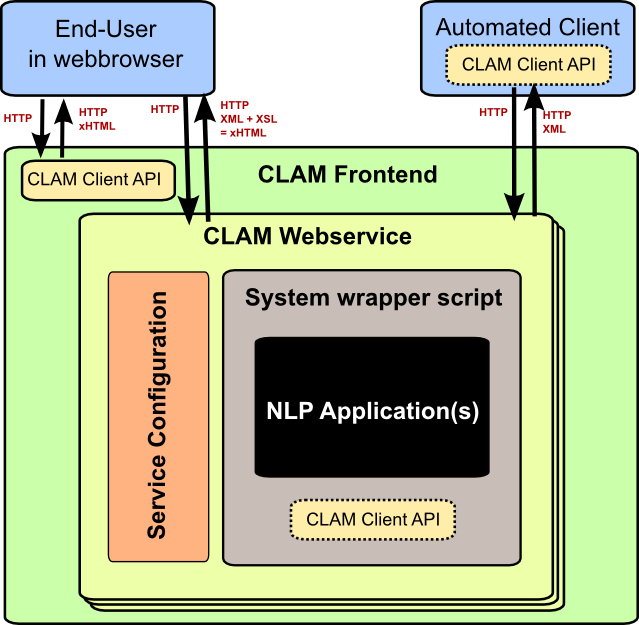
\includegraphics[width=70.0mm]{architecture.png}
        \end{center}
        \caption{The CLAM Architecture}
        \label{fig:arch} 
        \end{figure}


    \end{block}

\end{frame}



\subsection{Resource-oriented}
\begin{frame}

    \begin{block}{Resource oriented}
   
        \begin{itemize}
            \item Project
            \begin{itemize}
                \item Input files
                \begin{itemize}
                    \item Per-file parameter selection (=metadata)
                \end{itemize}
                \item Global system-wide parameter selection
                \item Output files
            \end{itemize}
        \end{itemize}

    \end{block}

    \begin{example}
        \B{Project example:} User wants to PoS-tag a corpus and starts a project for it \\
        \I{Input:} The untagged corpus \\
        \I{Output:} The tagged corpus \\
    \end{example}

\end{frame}


\section{Technical Details}

\begin{frame}{Technical Details}


    \begin{block}{RESTful Webservice}
        
        RESTful Webservice (as opposed to SOAP, XML-RPC)

        \begin{enumerate}
            \item Resource-oriented: "Representations" of "resources" (projects)
            \item Using HTTP verbs
            \item Lightweight
            \item Returns human-readable, machine-parseable XML adhering to a CLAM XML Scheme Definition %TODO: XSD not written yet
            \item User authentication in the form of HTTP Digest Authentication
        \end{enumerate}    
    \end{block}
\end{frame}

\begin{frame}
    \begin{block}{Python}
            Written entirely in Python 2.5

            \begin{enumerate}
                \item NLP tools, wrapper scripts, and clients may be in any language 
                \item But: Readily available API  when writing wrapper scripts and clients in Python.
                \item Built on web.py, runs standalone and out-of-the box with built-in CherryPy webserver        
            \end{enumerate}

    \end{block}
\end{frame}


\begin{frame}
    \begin{block}{Built-in User Interface}

            User interface automatically generated from XML using XSLT (in browser)

            \begin{enumerate}
                \item Webservice \emph{directly} accessible from webserver
                \item Web 2.0 interface: xHTML Strict, jquery (javascript), AJAX, CSS
            \end{enumerate}

            %Insert user-interface screenshot?

    \end{block}
\end{frame}



\section{Setup}

\subsection{Setup}

\begin{frame}{Setup}
    \begin{block}{CLAM Setup}

            Projects are the main resources, users start a new project for each experiment/batch.
    
            \textbf{Three states}:

            \begin{itemize}
                \item \textbf{Status 0)} Parameter selection and file upload
                \item \textbf{Status 1)} System in progress
                \begin{itemize}
                    \item Actual NLP tool invoked at this stage only
                    \item Users may safely close browser, shut down computer, and come back later in this stage
                \end{itemize}
                \item \textbf{Status 2)} System done, view/download output files
            \end{itemize}

            %Insert user-interface screenshot?

    \end{block}
\end{frame}

\section{Providing a Service}

\subsection{Providing a Service}

\begin{frame}
    \begin{block}{Providing a Service (1/2)}
        In order to make a webservice: \\       
        \textbf{1)} Write a service configuration file
        \begin{itemize}
            \item General meta information about your system {\footnotesize{(name, description, etc..)}}
            \item Definition of global parameters accepted by your system {\footnotesize{(i.e. the wrapper script around your NLP tool)}}
            \item Definition of \emph{profiles}
            \begin{itemize}
                \item A profile defines in detail what output a system produces given a certain input.                    
            \end{itemize}
        \end{itemize}    
    
    \end{block}

\end{frame}            

\begin{frame}
    \begin{block}{Providing a Service (2/2)}
        In order to make a webservice: \\
        \textbf{2)} Write a wrapper script for your system
        \begin{itemize}
            \item Wrapper script is invoked by CLAM, and should in turn invoke the actual system
            \item Acts as glue between CLAM and your NLP Application.
            \item Can be written in any language (python users may benefit from the CLAM API)
            \item Not always necessary, NLP applications can be invoked directly by CLAM as well.
        \end{itemize}
    
    \end{block}

\end{frame}

\subsection{Profiles}

\begin{frame}
    \begin{block}{Profiles}    
        Profiles define...
        \begin{itemize}
            \item \textbf{... what output files are produced given which input files}
            \item ... what metadata parameters are required or possible on input files
            \item ... how metadata fields are propagated from input files to output files
            \item ... what viewers are associated with output files (for webapplication)
            \item ... which converters can act upon input/output files (for webapplication)
        \end{itemize}        
    \end{block}
\end{frame}

\begin{frame}
    \begin{block}{Profiles}    
        Profiles define what output files are produced given which input files
        \begin{itemize}
            \item Input Templates
            \item Output Templates
            \begin{itemize}
                \item An output template may be conditional on global parameters
            \end{itemize}
        \end{itemize}        
    \end{block}
    
\end{frame}

\begin{frame}

Metaphore:
\begin{center}
\includegraphics[width=90.0mm]{blokkendoos.jpg}
\end{center}

\end{frame}

\begin{frame}
    \begin{example}
        Profile examples: 
        
        \begin{enumerate}
            \item A machine translation system:
            \begin{itemize}
                \item \textbf{Input Template: } The input text in source language X which is to be translated
                \item \textbf{Output Template: } The translated text target language Y
            \end{itemize}    
            \item A simple lexicon-based spelling correction system:
            \begin{itemize}
                \item \textbf{Input Template: } The input text which is to be corrected
                \item \textbf{Input Template: } A lexicon
                \item \textbf{Output Template: } The corrected text
            \end{itemize}    
        \end{enumerate}
        
    \end{example}
\end{frame}

\subsection{Writing a Wrapper Script}

\begin{frame}
    \begin{block}
        Typical layout of a wrapper script:
        \begin{enumerate}
            \item Read command line arguments (argv) set by CLAM
            \begin{itemize}
                \item Typical arguments are: Input Directory, Output Directory, Clam XML file            
            \end{itemize}
            \item Parse Clam XML file (easy using CLAM Data API)
            \item Read user-set parameters and iterate over input files, do whatever you need to do
            \item Invoke your NLP tool (system call)                
        \end{enumerate}
    \end{block}
\end{frame}        

\section{Writing a Client}

\begin{frame}
    \begin{block}{Writing a Client to connect to an existing service}
        \begin{enumerate}
            \item Communicate with service over HTTP, using HTTP verbs on projects and files to effectuate state transfers 
            {\footnotesize
            \begin{itemize}
                \item \texttt{GET /} - List all projects
                \item \texttt{GET /\{project\}/} - Get a project's current state (CLAM XML)
                \item \texttt{PUT /\{project\}/} - Create a new empty project
                \item \texttt{POST /\{project\}/} - Start a project with POSTed data as parameters
                \item \texttt{DELETE /\{project\}/} - Delete or abort a project
                \item \texttt{POST /\{project\}/input/\{filename\}} - Upload input file
                \item \texttt{GET /\{project\}/output/} - Download all output files as archive
                \item \texttt{GET /\{project\}/output/\{filename\}} - Download output file
            \end{itemize}
            }
            \item Check HTTP return codes and parse XML responses
        \end{enumerate}
    \end{block}

\end{frame}


\begin{frame}
    \begin{block}{Writing a Client to connect to an existing service}
        Python users benefit from CLAM Client API, taking care of all communication and response parsing!
    \end{block}

\end{frame}

\section{End}


\begin{frame}
    \raccoon
\end{frame}



\end{document}
